\documentclass[border=10pt]{standalone}
\usepackage{pgfplots}
\pgfplotsset{compat=1.18}
\begin{document}
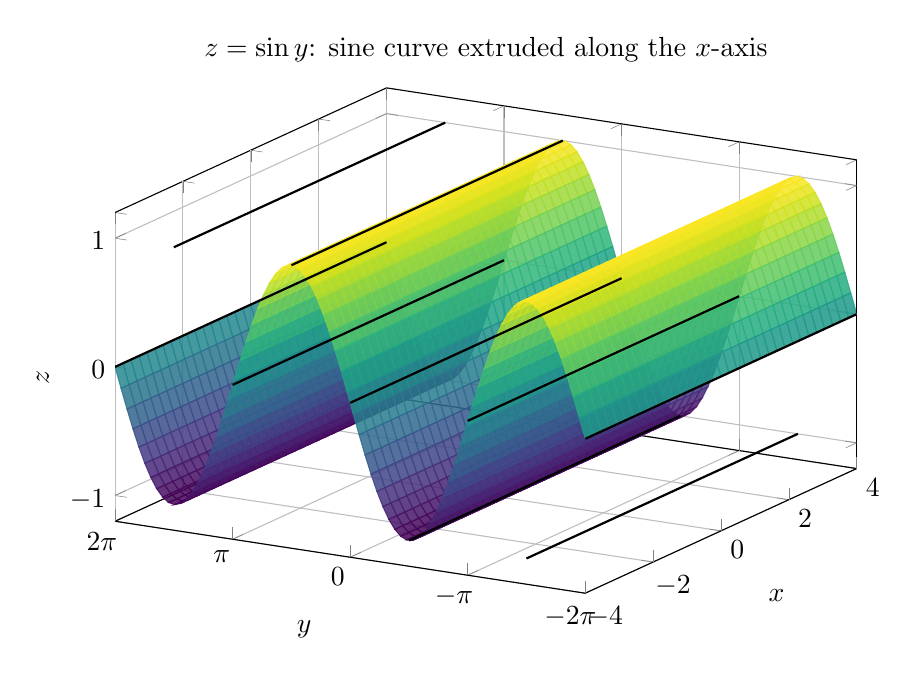
\begin{tikzpicture}
\begin{axis}[
  width=11cm, height=8cm,
  xlabel={$x$}, ylabel={$y$}, zlabel={$z$},
  title={$z=\sin y$: sine curve extruded along the $x$-axis},
  domain=-4:4,
  y domain=-2*pi:2*pi,
  samples=35,
  samples y=80,
  view={-60}{25},
  ztick={-1,0,1},
  ytick={-6.283,-3.142,0,3.142,6.283},
  yticklabels={$-2\pi$,$-\pi$,$0$,$\pi$,$2\pi$},
  grid=major,
  colormap/viridis,
]
\addplot3[surf,shader=flat,opacity=0.85] {sin(deg(y))};
% Rulings parallel to x-axis at key y-values
\addplot3[domain=-4:4, samples=2, black, thick] ({x}, {-2*pi}, {0});
\addplot3[domain=-4:4, samples=2, black, thick] ({x}, {-3*pi/2}, {-1});
\addplot3[domain=-4:4, samples=2, black, thick] ({x}, {-pi}, {0});
\addplot3[domain=-4:4, samples=2, black, thick] ({x}, {-pi/2}, {-1});
\addplot3[domain=-4:4, samples=2, black, thick] ({x}, {0}, {0});
\addplot3[domain=-4:4, samples=2, black, thick] ({x}, {pi/2}, {1});
\addplot3[domain=-4:4, samples=2, black, thick] ({x}, {pi}, {0});
\addplot3[domain=-4:4, samples=2, black, thick] ({x}, {3*pi/2}, {1});
\addplot3[domain=-4:4, samples=2, black, thick] ({x}, {2*pi}, {0});
\end{axis}
\end{tikzpicture}
\end{document}